\documentclass[a4paper,10pt,fleqn]{article}

\usepackage{../layout/layout}
\usepackage{pdfpages}
\title{Projektmanagementplan}

\begin{document}

% Eigene Titelseite
    \begin{titlepage}
        \begin{center}
            \makeatletter
            {\Large Produktentwicklung 1} \\
            \vfill{}
            {\LARGE \@title}
            \vfill{}
            {Team 27 \\
            Yannik Küng \\
            Andriu Maissen \\
            Daniel Mathis \\
            Simon Neidhart \\
            Peter Kounen \\
            Kevin Wespi \\
            Daniel Winz}
            \vfill{}
            {Betreuender Dozent: \\
            Marco De Angelis}
            \vfill{}
            {Hochschule Luzern \\
            Technik \& Architektur}
            \vfill
            {\today \\
            Git revision: 
            \input{../../.git/ORIG_HEAD}}
            \makeatother
        \end{center}
    \end{titlepage}

%\prentitle     % not yet working. -> See ../layout/layout.sty for details
\clearpage
\tableofcontents
\clearpage

\newcommand{\tabheader}     % Tabellenkopf
{
    \begin{zebratabular}[l]{@{}p{0.2\linewidth}p{0.3\linewidth}p{0.3\linewidth}p{0.06\linewidth}@{}}
    \rowcolor{gray}
    Stichwort &
        Quelle &
        Beschreibung &
        Bew. \\
}



	\section{Organigramm}
	\begin{figure}[hb]
		\centering
		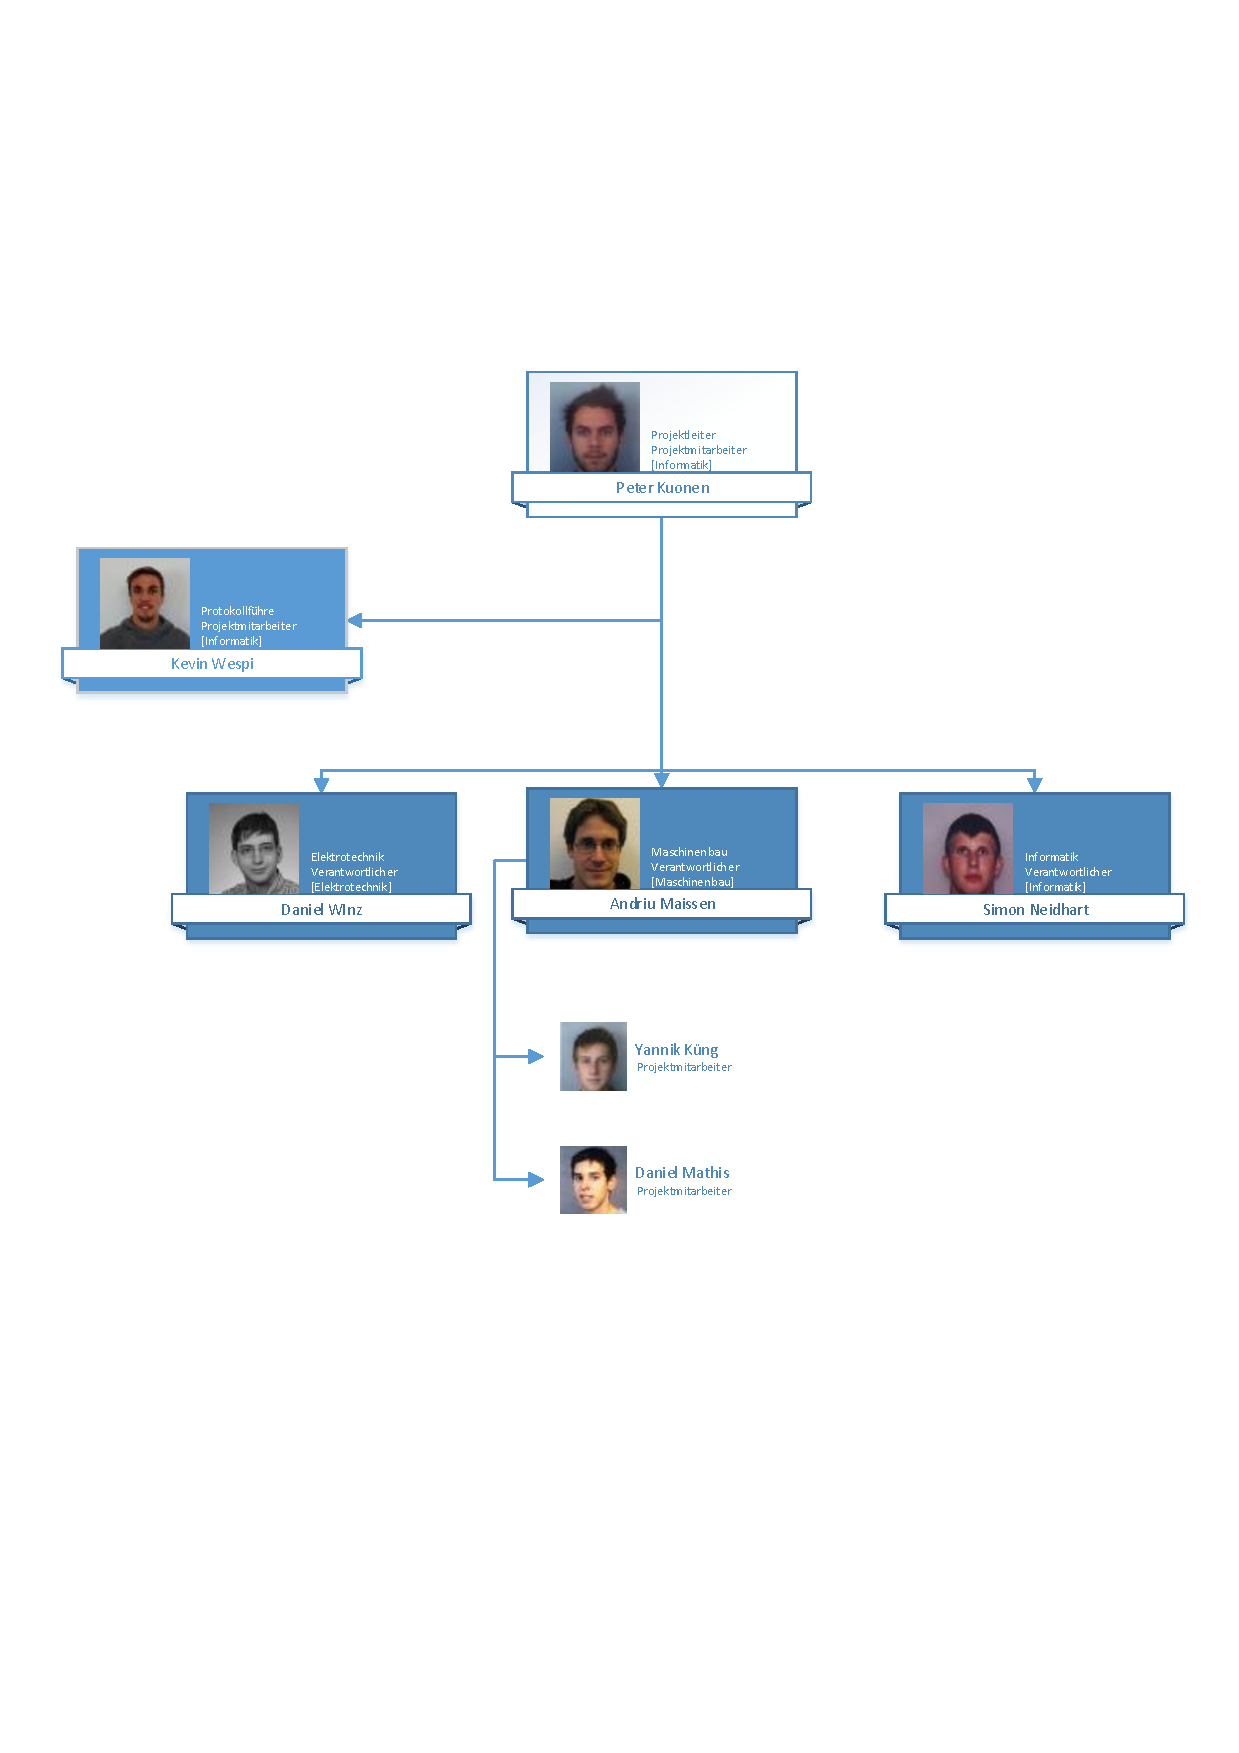
\includegraphics[width=4.5in]{pdf/organigramm.pdf}
	\end{figure}

	\section{Projektauftrag}
	Das Projekt PREN1 beschäftigt sich damit, einen Roboter zu bauen, der Autonom 5 Tennisbälle in einen Korb legt. Dazu ist ein Spielfeld vorgegeben und einige Kriterien welche in den Projektanforderungen beschrieben sind.
		
	\section{Projektterminplan}
	Hier folgt der Projektterminplan (grafische Darstellung)
	
	\section{Risikomanagement}
	Hier folgt das Risikomanagement
	
	\section{Workplace Beschreibung}
	Hier folgt eine Auflistung, was für Programme / Betriebssysteme und auch Maschinen von wem benutzt werden. Um die Aufgabe zu erfüllen.
	
	\section{Testumgebung}
	Hier folgt ein Beschrieb wie wir gedenken verschiedene Teile des Projektes zu testen.
	
	


\end{document}
